\section{Solution réalisée}
Une étape essentielle dans tout système électrique réside premièrement dans son câblage. Le but est de réaliser un câblage le plus propre et pratique possible. La figure \ref{cablage_kit_pas_annoté}, ci-dessous, est une photo du kit sans les annotations afin que le câblage effectué soit plus visible. On retrouve cette même photo, sur la page suivante, avec les annotations et les explications en détail des différents câbles.
\begin{figure}[H]
    \begin{center}
        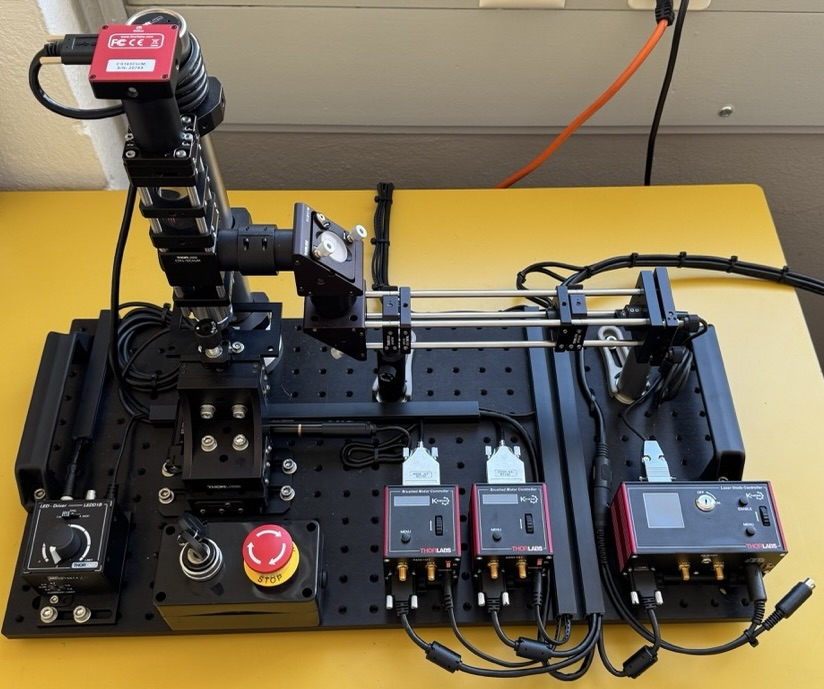
\includegraphics[width=\textwidth]{assets/figures/Cablage_du_kit/Cablage_vierge.jpeg}
    \end{center}
    \caption{Câblage du kit sans annotations}
    \label{cablage_kit_pas_annoté}
\end{figure}

\newpage
Ci-dessous, une photo du câblage avec des annotations pour une bonne compréhension du travail réalisé (voir Figure \ref{cablage_kit_annoté}).


\begin{figure}[H]
    \begin{center}
        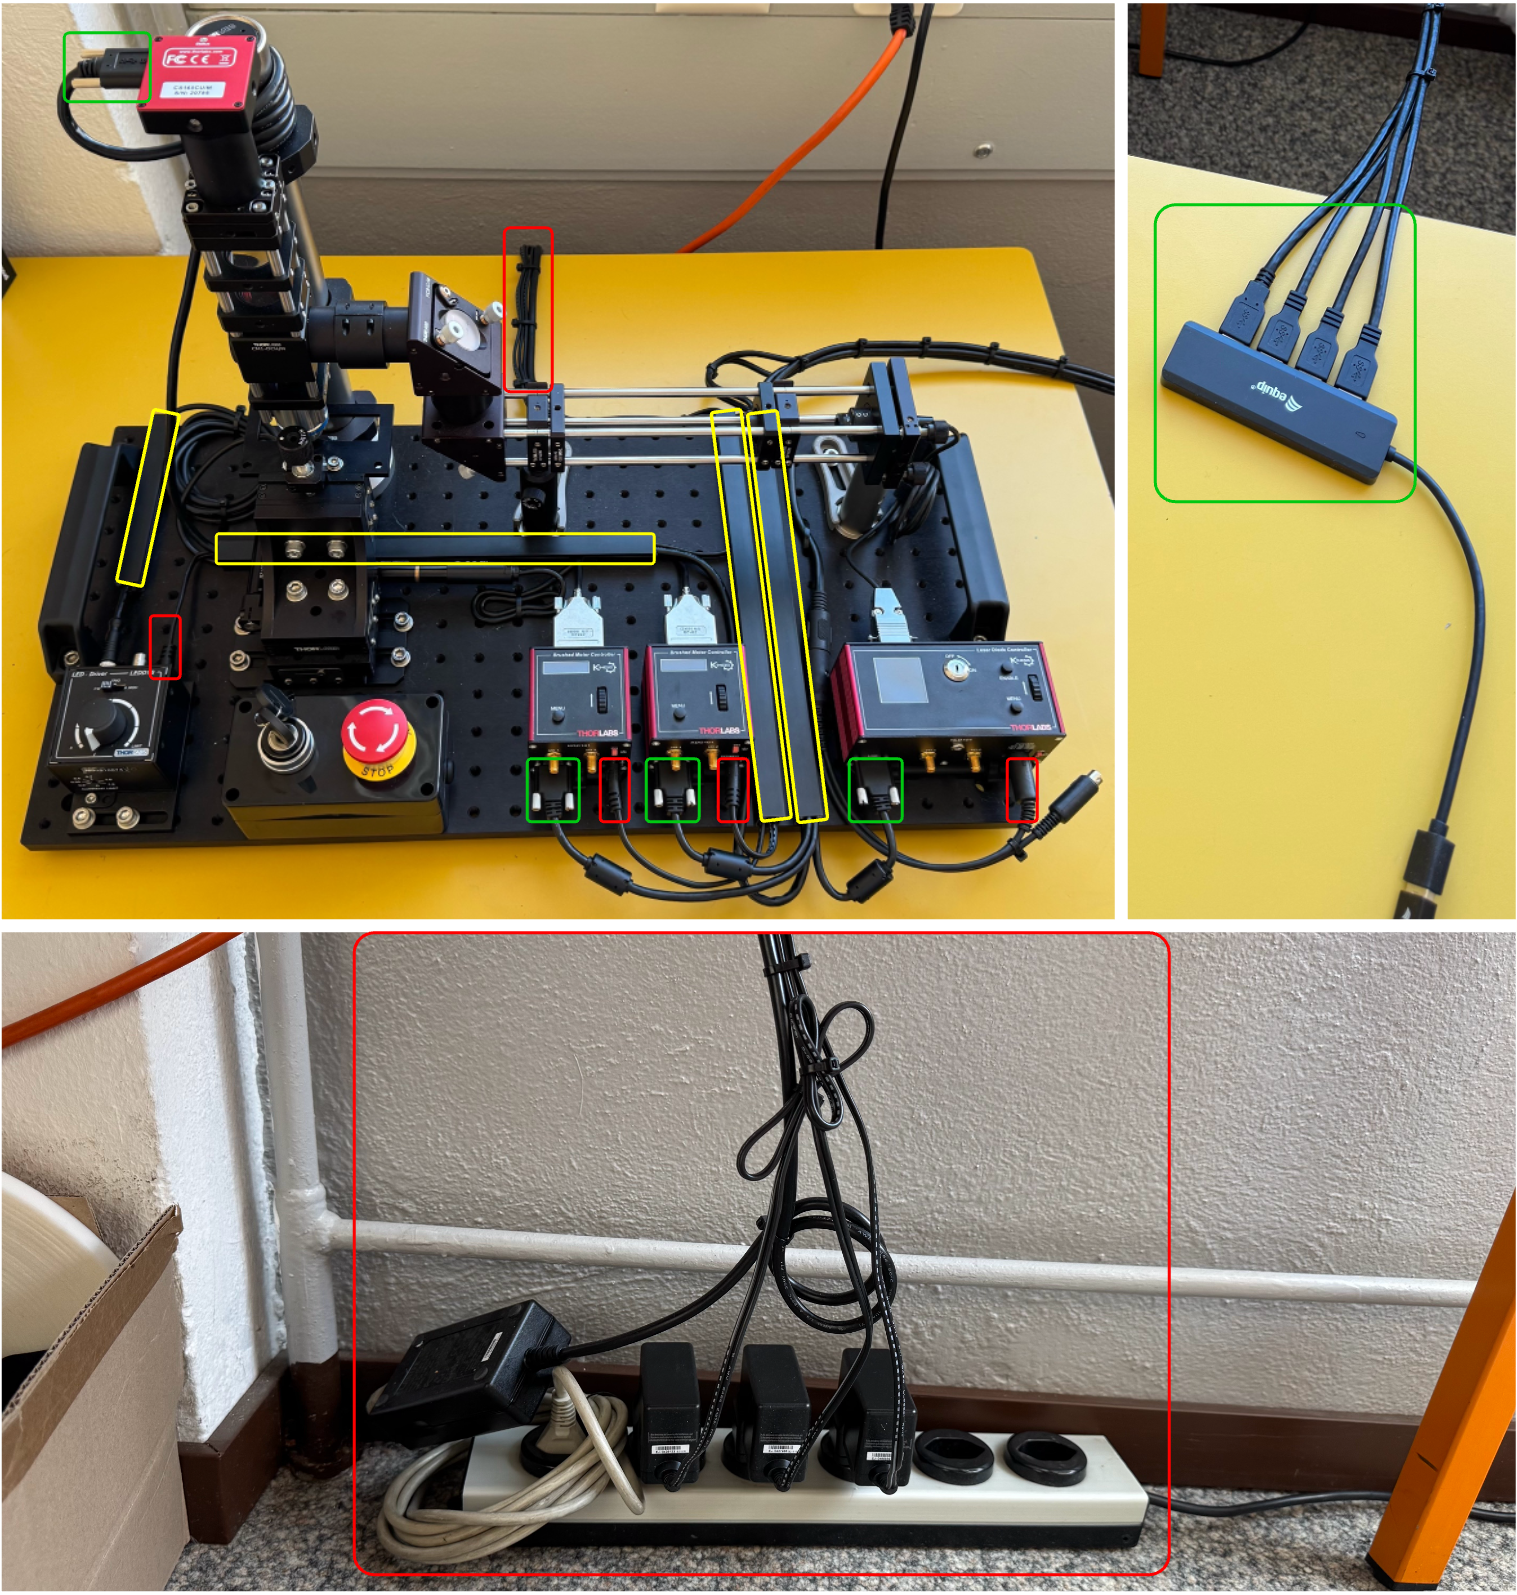
\includegraphics[width=0.9\textwidth]{assets/figures/Cablage_du_kit/Cablage_annote.png}
    \end{center}
    \caption{Câblage du kit avec annotations}
    \label{cablage_kit_annoté}
\end{figure}

On peut apercevoir en \textcolor[RGB]{230, 230, 0}{jaune}, que des goulottes ont été installées afin que les câbles tiennent en place, mais également afin d'avoir un visuel au propre.

Les encadrés en \textcolor{red}{rouge} sont les quatres alimentations. Celles-ci sont utilisées pour :
\begin{itemize}
    \item Les deux drivers des servomoteurs
    \item Le driver du laser
    \item Le driver de la LED
\end{itemize}

En complément des alimentations, les encadrés en \textcolor[RGB]{0, 201, 18}{vert} désignent les câbles permettant de communiquer avec les différents composants. Voici, ci-dessous, la liste des câbles pour la communication :
\begin{itemize}
    \item Un câble pour chaque driver de servomoteur, deux au total
    \item Un câble pour le driver du laser
    \item Un câble pour la caméra
\end{itemize}